%%%%%%%%%%%%%%%%%%%%%%%%%%%%%%%%%%%%%%%%%
% Short Sectioned Assignment LaTeX Template Version 1.0 (5/5/12)
% This template has been downloaded from: http://www.LaTeXTemplates.com
% Original author:  Frits Wenneker (http://www.howtotex.com)
% License: CC BY-NC-SA 3.0 (http://creativecommons.org/licenses/by-nc-sa/3.0/)
%%%%%%%%%%%%%%%%%%%%%%%%%%%%%%%%%%%%%%%%%

%----------------------------------------------------------------------------------------
%	PACKAGES AND OTHER DOCUMENT CONFIGURATIONS
%----------------------------------------------------------------------------------------

\documentclass[paper=a4, fontsize=11pt]{scrartcl} % A4 paper and 11pt font size

% ---- Entrada y salida de texto -----

\usepackage{hyperref}
\usepackage{varioref}
\usepackage[T1]{fontenc} % Use 8-bit encoding that has 256 glyphs
\usepackage[utf8]{inputenc}
%\usepackage{fourier} % Use the Adobe Utopia font for the document - comment this line to return to the LaTeX default

% ---- Idioma --------

\usepackage[spanish, es-tabla]{babel} % Selecciona el español para palabras introducidas automáticamente, p.ej. "septiembre" en la fecha y especifica que se use la palabra Tabla en vez de Cuadro

% ---- Otros paquetes ----

\usepackage{amsmath,amsfonts,amsthm} % Math packages
%\usepackage{graphics,graphicx, floatrow} %para incluir imágenes y notas en las imágenes
\usepackage{graphics,graphicx, float} %para incluir imágenes y colocarlas

% Para hacer tablas comlejas
%\usepackage{multirow}
%\usepackage{threeparttable}

%\usepackage{sectsty} % Allows customizing section commands
%\allsectionsfont{\centering \normalfont\scshape} % Make all sections centered, the default font and small caps

\usepackage{fancyhdr} % Custom headers and footers
\pagestyle{fancyplain} % Makes all pages in the document conform to the custom headers and footers
\fancyhead{} % No page header - if you want one, create it in the same way as the footers below
\fancyfoot[L]{} % Empty left footer
\fancyfoot[C]{} % Empty center footer
\fancyfoot[R]{\thepage} % Page numbering for right footer
\renewcommand{\headrulewidth}{0pt} % Remove header underlines
\renewcommand{\footrulewidth}{0pt} % Remove footer underlines
\setlength{\headheight}{13.6pt} % Customize the height of the header

\numberwithin{equation}{section} % Number equations within sections (i.e. 1.1, 1.2, 2.1, 2.2 instead of 1, 2, 3, 4)
\numberwithin{figure}{section} % Number figures within sections (i.e. 1.1, 1.2, 2.1, 2.2 instead of 1, 2, 3, 4)
\numberwithin{table}{section} % Number tables within sections (i.e. 1.1, 1.2, 2.1, 2.2 instead of 1, 2, 3, 4)

\setlength\parindent{0pt} % Removes all indentation from paragraphs - comment this line for an assignment with lots of text

\newcommand{\horrule}[1]{\rule{\linewidth}{#1}} % Create horizontal rule command with 1 argument of height


%----------------------------------------------------------------------------------------
%	TÍTULO Y DATOS DEL ALUMNO
%----------------------------------------------------------------------------------------

\title{	
\normalfont \normalsize 
\textsc{{\bf Ingeniería de Servidores (2015-2016)} \\ Grado en Ingeniería Informática \\ Universidad de Granada} \\ [25pt] % Your university, school and/or department name(s)
\horrule{0.5pt} \\[0.4cm] % Thin top horizontal rule
\huge Memoria Práctica 1 \\ % The assignment title
\horrule{2pt} \\[0.5cm] % Thick bottom horizontal rule
}

\author{Francisco Carrillo Pérez} % Nombre y apellidos

\date{\normalsize\today} % Incluye la fecha actual

%----------------------------------------------------------------------------------------
% DOCUMENTO
%----------------------------------------------------------------------------------------

\begin{document}

\maketitle % Muestra el Título

\newpage %inserta un salto de página

\tableofcontents % para generar el índice de contenidos

\listoffigures

\listoftables

\newpage


%----------------------------------------------------------------------------------------
%	Cuestión 1
%----------------------------------------------------------------------------------------

\section{Cuestión 1: ¿Qué modos y/o tipos de virtualización existen? }

Hay dos tipos de virtualización: \cite{virtual} \cite{ibmvirtualization}

\begin{itemize}
	\item \textbf{Hardware Virtualization: } Consiste en la construcción de una máquina virtual,que actúa como un ordenador real con un sistema operativo. El software usado en estas máquinas virtuales está separado de los recursos hardware que van por debajo.\\
	Dentro de la Hardware Virtualization hay tres tipos:
	\begin{itemize}
		\item \textbf{Virtualización total: } casi una completa simulación del hardware que permite al software ejecutarse sin modificar.
		\item \textbf{Virtualización parcial: } algunos pero no todos los atributos son simulados. Como resultado, algunos programas necesiten modificaciones para ejecutarse en estos entornos virtuales.
		\item \textbf{Paravirtualización: } el entorno hardware no se simula; de todas formas, los programas huéspedes son ejecutados como si se ejecutaran en sistema a parte. Los programas huéspedes necesitan ser específicamente modificados para poder ejecutarse.
	\end{itemize}
	\item \textbf{Desktop Virtualization: } consisten en separar el escritorio lógico de la parte física de la máquina. Una forma de Desktop Virtualization ,VDI (Virtual Desktop Infraestructure), puede verse como una forma más avanzada de Hardware Virtualization. Más que interactuar con la máquina anfitriona directamente vía teclado, ratón y monitor, el usuario interactúa con la máquina anfitriona usando otro escritorio de ordenador o dispositivo móvil con una conexión de red, ya sea LAN, Wireless LAN o incluso Internet. Por ejemplo, compañías como HP o IBM  proveen un modelo VDI híbrido con variedad de Virtualization Software y modelos de envío que mejoran las limitaciones de la computación distribuida.
\end{itemize}


%----------------------------------------------------------------------------------------
%	Cuestión 2
%----------------------------------------------------------------------------------------

\section{Cuestión 2: Muestre los precios y características de varios proveedores de VPS(Virtual Private Service) y compare con el precio  de servidores dedicados (administrados y no administrados). Comente las diferencias}

\textbf{VPS}\\
\begin{itemize}
	\item \textbf{Hostalia: \cite{hostalia}} Esta empresa ofrece tres paquetes:\\ \label{host}
	\begin{itemize}
		\item \textbf{VPS Base: } desde 11,21 euros/mes ofrece 25 GB de espacio en disco,  1GB de memoria RAM y 1000GB de transferencia.
		\item \textbf{VPS Avanzado: } desde 18.71 euros/mes ofrece 50GB de espacio de disco, 2GB de memoria RAM y 1000GB de transferencia.
		\item \textbf{VPS Plus: } desde 26.21 euros/mes ofrece 100GB de espacio en disco, 3GB de memoria RAM y 1000GB de transferencia.
	\end{itemize}
	\item \textbf{DigitalOcean: \cite{digitalocean}} La empresa DigitalOcean ofrece varios paquetes:\\ \label{dg}
	\begin{itemize}
		\item 5 dólares/mes(4,47962 euros/mes \cite{divisas}) : 512 MB de memoria RAM, 1 core, 20GB SSD y  1TB de transferencia.
		\item 10 dólares/mes(8,95887 euros/mes) : 1GB de memoria RAM, 1 core, 30 GB SSD y 2TB de transferencia.
		\item 20 dólares/mes(17,9177 euros/mes) : 2GB de memoria RAM, 2 core, 40GB SSD y 3TB de transferencia.
		\item 40 dólares/mes(35,8355 euros/mes) : 4GB de memoria RAM, 2 core, 60GB SSD y 4TB de transferencia.
		\item 80 dólares/mes(71,6767 euros/mes) : 8GB de memoria RAM, 5 core, 80GB SSD y 5TB de transferencia.
	\end{itemize}
	
\textbf{Servidores dedicados}\\
\begin{itemize}
	\item \textbf{1and1: \cite{1and1}} La empresa 1and1 ofrece varios paquetes: \label{1a1} 
		\begin{itemize}
			\item 39,99 euros/mes: Procesador:AMD Quad-Core;Núcleos de CPU: 4 Cores x 2.1 GHz; Memoria RAM: 4 GB DDR2;Disco Duro: 750 GB
			(2 x 750 GB SATA);RAID:Software RAID 1.
			\item 79.99 euros/mes: Procesador:AMD Hexa-Core;Núcleos de CPU: 6 Cores x 2.8 GHz (3.3 GHz Turbo Core); Memoria RAM: 16 GB
			DDR3 ECC DDR2;Disco Duro: 1,000 GB (2 x 1,000 GB SATA);RAID:Software RAID 1.
			\item 59,99 euros/mes:  Procesador:Intel®Atom™ C2750;Núcleos de CPU: 8 Cores x 2,4 GHz(2,6 GHz Turbo Boost); Memoria RAM: 8 GB de RAM DDR3 ECC;Disco Duro: 1,000 GB (2 x 1,000 GB SATA);RAID:Software RAID 1. 
			\item 119,99 euros/mes: Procesador:AMD Opteron™ 4274 HE;Núcleos de CPU: 8 Cores x 2,6 GHz(3.5 GHz Turbo Boost); Memoria RAM: 16 GB de RAM DDR3 ECC;Disco Duro: 1,500 GB (2 x 1,500 GB SATA);RAID:Software RAID 1.
			\item 79,99 euros/mes: Procesador:Intel®Xeon® E3-1270 V3;Núcleos de CPU:4 Cores (HT) x 3,5 GHz; Memoria RAM: 16 GB de RAM DDR3 ECC;Disco Duro: 1,000 GB (2 x 1,000 GB SATA);RAID:Software RAID 1. \label{80euros}
		\end{itemize}
\end{itemize} 
\textbf{Comentarios}\\
Como se puede observar, hay claras diferencias entre los servicios que nos ofrecen. En cuanto a los VPS tenemos en muchos casos menos potencia, en el mismo rango de precios. Por ejemplo vamos a observar las diferencias primero entre los dos servicios de VPS de DigitalOcean \vref{dg} y Hostalia \vref{host}. El servicio de 17,9177 euros/mes de DigitalOcean nos ofrece 2GB de RAM, lo mismo que el de Hostalia, 2 core, no hay información de Hostalia al respecto, 40GB SSD, frente a los 50 GB SSD de Hostalia, y 2TB de transferencia, frente a las 1000GB de Hostalia. Como podemos observar los precios son bastante parecidos, los diferencian datos como la transferencia, y el almacenamiento, Hostalia tiene 10GB más que DigitalOcean. \\
Ahora, si miramos la diferencia entre por ejemplo el VPS de DigitalOcean \vref{dg} y el servidor dedicado de 1and1 \vref{1a1}, veremos claras diferencias. Si miramos la tarifa de 1and1 de 80euros/mes \vref{80euros} y la de DigitalOcean de 71 euros/mes (se que la diferencia de precio es notable, pero no se puede hacer otra comparativa en cuanto a rangos de precios), podemos observar que hay diferencias notables, tanto en RAM como en Disco Duro, y núcleos de la CPU. 

\end{itemize}

\section{Cuestión 3: ¿Qué otros software de virtualización existen además deVMWare y Virtual Box?}
Existen diferentes alternativas: \cite{similar2vmw}
\begin{itemize}
	\item QEMU (Mac OS, Windows, Linux, BSD)
	\item Parallels Desktop (Mac OS)
	\item Paragon Virtualization Manager (Linux)
\end{itemize}

\section{Cuestión 4: Enumere algunas de las innovaciones en Windows 2012 R2 respecto a 2008R2 }

\begin{figure}[H] %con el [H] le obligamos a situar aquí la figura
	\centering
	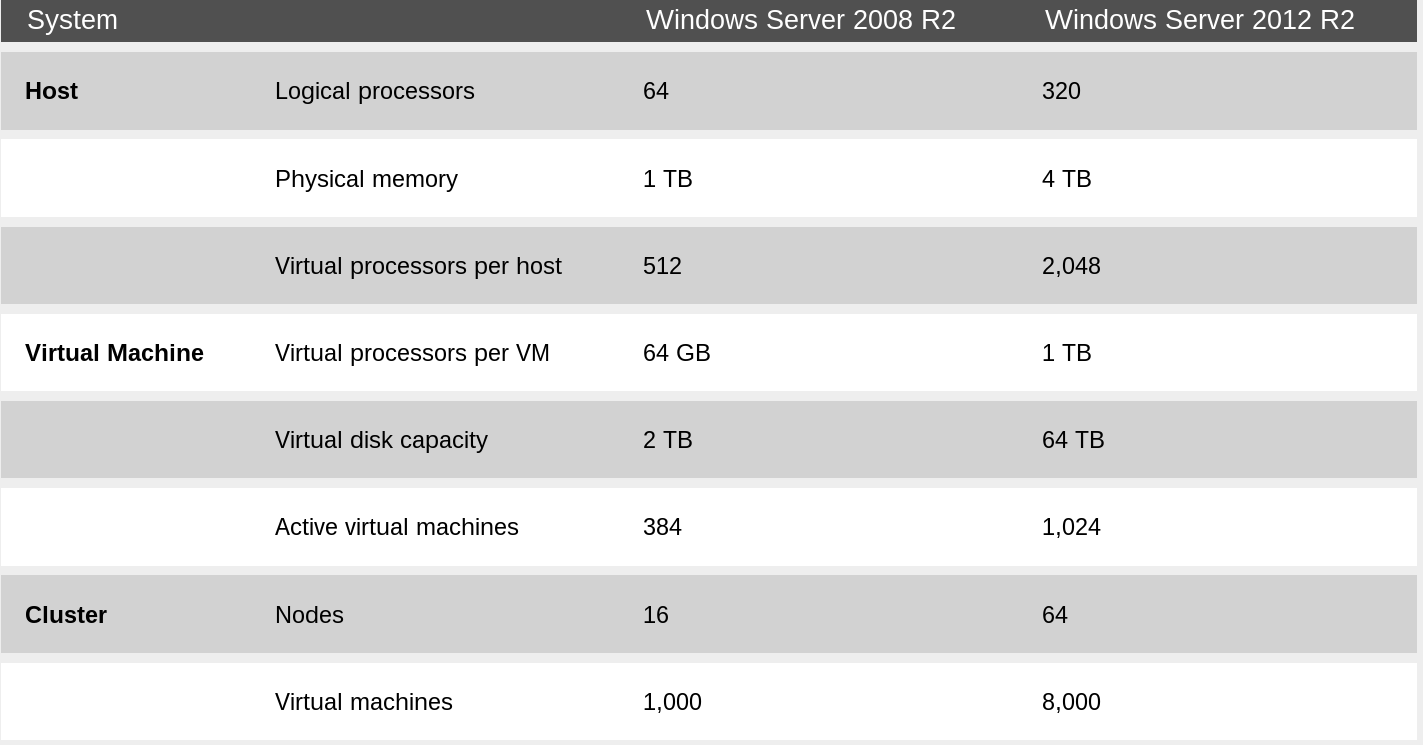
\includegraphics[scale=0.3]{figuras/figura1.png}  %el parámetro scale permite agrandar o achicar la imagen. En el nombre de archivo puede especificar directorios
	\label{figura1}
	
	\caption{Tabla de las innovaciones de Windows 2012R2 con Windows 2008R2 \cite{windows2012vs2008}} 
\end{figure}

Cómo podemos observar en la tabla de la figura 1 \ref{figura1} las diferencias entre Windows 2008 y 2012 son:\\
Tenemos mucha más memoria física, además de procesadores lógicos. Muchás más máquinas virtuales activas, y más nodos en los cluster.
\section{Cuestión 5: ¿Qué empresa hay detrás de Ubuntu? ¿Qué otros productos/servicios ofrece?}
La empresa que se encuentra detrás de Ubuntu es Canonical. 
\begin{figure}[H] %con el [H] le obligamos a situar aquí la figura
	\centering
	
\includegraphics[scale=0.3]{figuras/canonical.jpg}  %el parámetro scale permite agrandar o achicar la imagen. En el nombre de archivo puede especificar directorios
	\label{figura2}
	
	\caption{Logo de canonical \cite{logocano}} 
\end{figure}

Canonical tiene otros productos tales como: \cite{canonicalp}
\begin{itemize}
	\item \textbf{GNU Bazaar: } un sistema de revisión de control descentralizado.
	\item \textbf{Storm: } un objeto-relacional mapper para Python.
	\item \textbf{Juju: } una herramienta de gestión de orquestación de servicios.
	\item \textbf{Quickly: } un framework para la creación de programas software para Linux.
	\item \textbf{Ubiquity: } instalador de Ubuntu.
	\item \textbf{Mir: } servidor de pantalla.
	\item \textbf{Launchpad: } una página web centralizada que contienen varias herramientas que permiten la mejor colaboración de proyectos de software libre.
\end{itemize}

\section{Cuestión 6: ¿Qué relación tiene esta distribución (CentOS) con Red Hat y con el proyecto Fedora?}
CentOS es una distribución que lo que hace es que compila el código de RedHat ofreciendo una distribución libre de la misma, ya que hace varios años Red Hat hacía lo mismo que Ubuntu, tu pagabas por el soporte, pero hubo un punto de inflexión en que ya sólo se distrubuye el código fuente y si quiéres la ISO se envía en un DVD. En ese momento salió CentOS, para ofrecerlo libre, compilando todo el código, y ofreciendo uan distribución muy parecida a Red Hat. \cite{centOS} Aunque a partir del 7 de Enero de 2014 se unió a Red Hat para que el proyecto avanzase más rápidamente. \cite{centOS2}

\section{Cuestión 7: Indique qué otros SO se utilizan en servidores y el porcentaje de uso}
Los sistemas basados en BSD y otros Unix son algunos que no hemos analizado, como por ejemplo Debian \cite{debian}, que en la que se basa Ubuntu. Dentro de estos se encuentra por ejemplo \textbf{FreeBSD} que según su página web \cite{freebsd} : \textquotedblleft es un avanzado sistema operativo para arquitecturas x86 compatibles (como Pentium® y Athlon™), amd64 compatibles (como Opteron™, Athlon™64 EM64T), UltraSPARC®, IA-64, PC-98 y ARM. FreeBSD es un derivado de BSD, la versión de UNIX® desarrollada en la Universidad de California, Berkeley.\textquotedblright\\
También hay otros sistemas como \textbf{OS X Server} que según su página web \cite{osxserver}:  \textquotedblleft OS X Server es perfecto para estudios pequeños, pymes o centros escolares. Es tán fácil de usar que no hace falta un departamento de informática \textquotedblright.\\
O por ejemplo \textbf{Debian} \cite{debian}. \\ 
En la siguiente figura podemos ver los porcentajes de uso:

\begin{figure}[H] %con el [H] le obligamos a situar aquí la figura
	\centering
	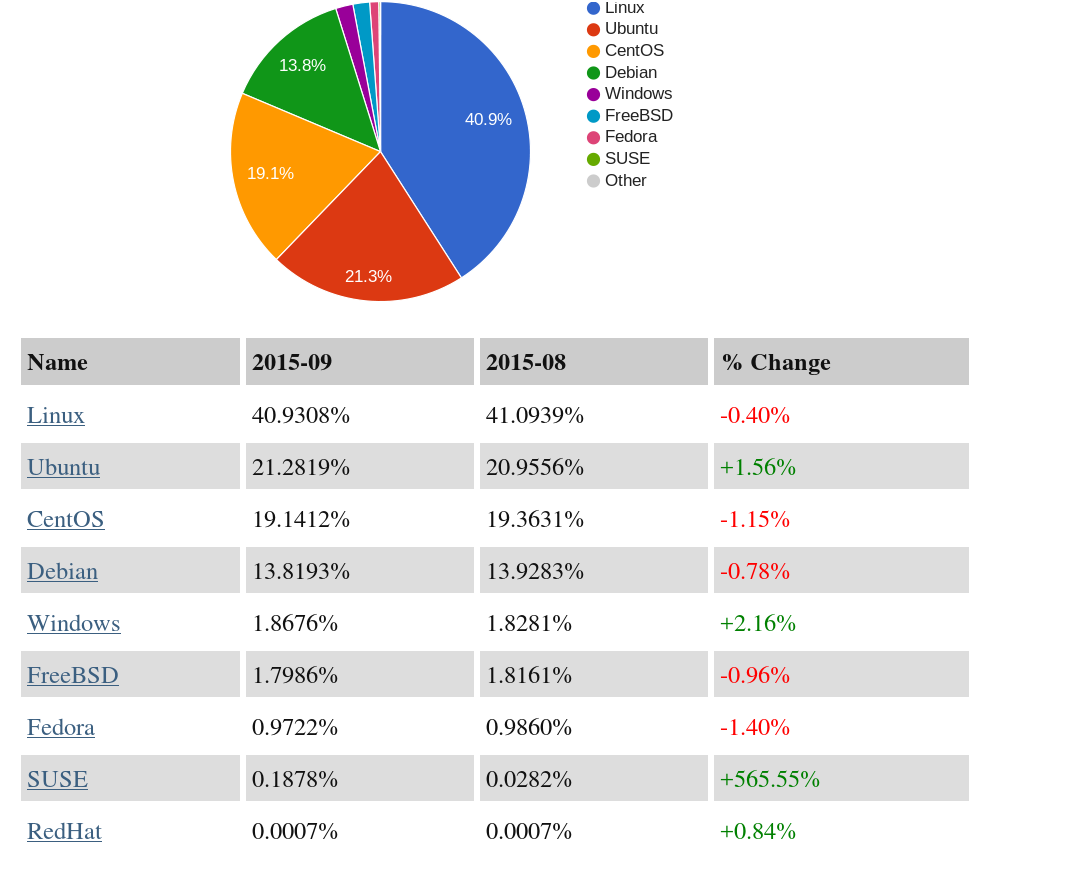
\includegraphics[scale=0.3]{figuras/figura3.png}  %el parámetro scale permite agrandar o achicar la imagen. En el nombre de archivo puede especificar directorios
	\label{figura3}
	
	\caption{Porcentaje de uso de los distintos SO en servidores \cite{perserv}} 
\end{figure}

\section{Cuestión 8:¿Qué diferencia hay entre RAID mediante SW y mediante HW?}
Según el artículo de la empresa Adaptec\cite{adaptec} sobre las diferencias del RAID mediante SW y el RAID mediante HW \cite{raidswhw}:
En el Raid mediante software la tarea del RAID corre en la CPU del sistema en cambio RAID mediante HW tiene su propio procesador y memoria donde corre el proceso del RAID. A veces algunas de las implementaiones SW del RAID incluyen alguna parte de Hardware pero esto no lo hace implementación HW.

\begin{figure}[H] %con el [H] le obligamos a situar aquí la figura
	\centering
	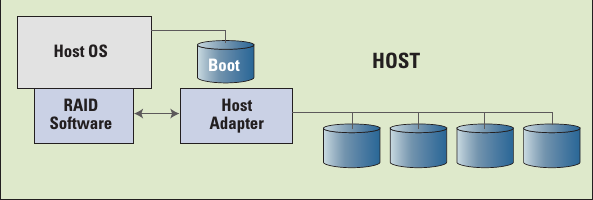
\includegraphics[scale=0.3]{figuras/figura4.png}  %el parámetro scale permite agrandar o achicar la imagen. En el nombre de archivo puede especificar directorios
	\label{figura4}
	
	\caption{RAID mediante SW. Figura del paper \cite{raidswhw}} 
\end{figure}
\begin{figure}[H] %con el [H] le obligamos a situar aquí la figura
	\centering
	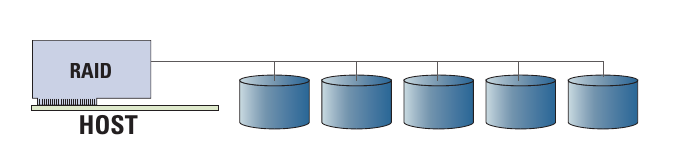
\includegraphics[scale=0.3]{figuras/figura5.png}  %el parámetro scale permite agrandar o achicar la imagen. En el nombre de archivo puede especificar directorios
	\label{figura5}
	
	\caption{RAID mediante HW. Figura del paper \cite{raidswhw}} 
\end{figure}

\section{Cuestión 9}
\subsection{a) ¿Qué es LVM?}
LVM según la wiki de ArchLinux es \cite{lvm}:\\
\textquotedblleft es un administrador de volúmenes lógicos para el kernel de Linux. Maneja discos duros y dispositivos de almacenamiento similares. \textquotedblright
\subsection{¿Qué ventaja tiene para un servidor de gama baja?}
Según la página \cite{small}:\\
Gracias al LVM podemos redimensionar según nuestras necesidades el espacio de las distintas particiones lógicas que componen nuestro disco duro. Esto nos permite que a lo largo del tiempo, podamos administrar mejor la memoria de nuestro ordenador, adaptándose a nuestras necesidades.
\subsection{Si va a tener un servidor web, ¿le daría un tamaño grande o pequeño a /var?}
Según \cite{var}:\\
\textquotedblleft El sistema de archivos /var contiene datos que cambian cuando el sistema se ejecuta normalmente. Es específico para cada sistema y por lo tanto no es compartido a través de la red con otras computadoras.\textquotedblright

Por lo tanto, al compartirse en red será necesario que tenga un tamaño grande, acorde a lo que debería tener un servidor pequeño, más los archivos temporales que se guarden en él.

\section{Cuestión 10: ¿Debemos cifrar también el volumen que contiene el espacio para swap?¿y el volumen en el que  montaremos /boot?}
Según la documentación de FreeBSD \cite{swapencr} el swap:\\
Si tenemos un programa que utiliza contraseñas, mientras que estas estén en el disco duro están encripyadas, pero en el momento en que pasen a memoria swap, mientras estén ahí, serán vulnerables a poder ser vistas. Por ello es necesario cifrar también el volúmen que contiene el espacio para swap. 

Según \cite{boot} el /boot:\\
no debe encriptarse, aunque es posible realizarlo con herramientas, ya que si tenemos encriptado el /boot, necesita que se desencripte para poder cargar los bloques donde se contiene el sistema operativo pero no se puede cargar ningúna interfaz ya que no no está cargado el sistema operativo por lo que no se puede desencriptar el boot.

\section{Cuestión 11: ¿Qué otro tipo de usos de una partición le permite configurar e asistente de instalación? ¿Cuál es la principal diferencia entre ext4 y ext2?}

Las otras particiones según el instalador de Ubuntu Server son: 
\begin{figure}[H] %con el [H] le obligamos a situar aquí la figura
	\centering
	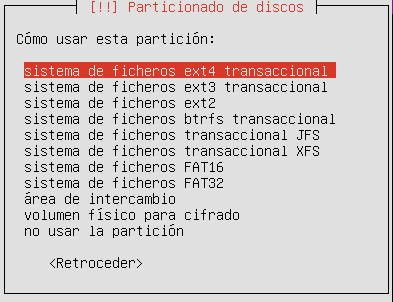
\includegraphics[scale=0.5]{figuras/figura7.png}  %el parámetro scale permite agrandar o achicar la imagen. En el nombre de archivo puede especificar directorios
	\label{figura7}
	
	\caption{Otros usos de partición en el instalador de Ubuntu Server \cite{ubuntuserver}} 
\end{figure}

La diferencia entre ext4 y ext2 es que \cite{ext2ext4}:
los dos, junto a ext3, son de la misma familia de sistemas de archivos. Lo que cambia son las extensiones que se añaden, ext3 tiene más extensiones que ext2 y ext4 más extensiones que ambos. Además utilizan las mismas utilidades del espacio de usuario por lo que algunos de sistemas de archivos pueden ser utilizados en otros sistemas de archivos. Un ext3 lo puedes montar en un ext4 pero un ext4 no puedes montarlo en un ext3 ni en un ext2.

\section{Cuestión 12: Muestre cómo ha quedado el disco particionado una vez el sistema está instalado}
El disco ha quedado:
\begin{figure}[H] %con el [H] le obligamos a situar aquí la figura
	\centering
	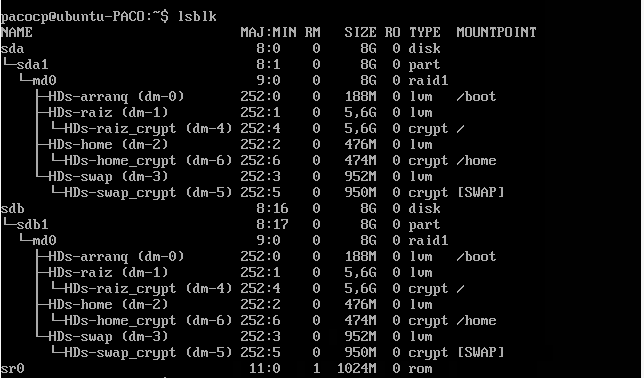
\includegraphics[scale=0.5]{figuras/figura6.png}  %el parámetro scale permite agrandar o achicar la imagen. En el nombre de archivo puede especificar directorios
	\label{figura6}
	
	\caption{Cómo queda el disco particionado en Ubuntu Server \cite{ubuntuserver}} 
\end{figure}

\section{Cuestión 13:}
\subsection{a) ¿Cómo ha hecho el disco 2 arrancable?}
He utilizado la instrucción grub-install según la página \cite{grub-install-gnu}:\\
\textbf{sudo grub-install /dev/sdb} \\
Al intentar arrancarlo ha surgido un bug. He seguido las siguientes instrucciones del profesor Alberto Guillén Perales \cite{alberto} para arreglarlo:
\begin{itemize}
	\item Miramos el archivo mdstat con: cat /proc/mdstat y comprobamos que el md0 se encuentra inativo.
	\item Mirando la página del man de la instrucción mdadm \cite{mdadm} debemos utilizar la opción -R para intentar activarlo: mdamd -R /dev/md0
	\item Por último, volvemos a mirar el archivo mdstat con: cat /proc/mdstat y comprobamos que el md0 ya se encuentra activo. Escribimos la instrucción exit y ya carga correctamente.
\end{itemize}
\subsection{b) ¿Qué hace el comando grub-install?}
Según la página del man en Ubuntu Server \cite{grub-install}:\\
\textquotedblleft Instala el GRUB en tu disco \textquotedblright
\subsection{c) ¿Qué hace el comando dd?}
Según la página del man en Ubuntu Server \cite{dd}:\\
\textquotedblleft Copia un archivo, lo convierte y lo transforma acorde a los operandos que se le pasen \textquotedblright
\section{Cuestión 14: ¿Qué diferencia hay entre Standard y Datacenter?}
Según indican los PDF que se puede descargar de la página de Windows (documentación y detallado de las ediciones) \cite{datacentervsstandar} \cite{datacentervsstandar2}:\\
Las únicas diferencias es que mientras en el Standard podemos correr a la vez sólo 4 instancias, en el Datacenter podemos correr tantas como queramos siempre bajo las limitaciones de los recursos. Además, mientras que activación automática de las máquinas virtuales en dataCenter se puede hacer tanto para host como para guest, en Standard solo se puede hacer para guest.

\section{Cuestion 15: Continúe usted con el proceso de definición de RAID1 para los dos discos de 50MBi que ha creado. Muestre el proceso con capturas de pantalla}
Con las siguientes capturas voy a describir el proceso de definición del RAID1:
\begin{figure}[H] %con el [H] le obligamos a situar aquí la figura
	\centering
	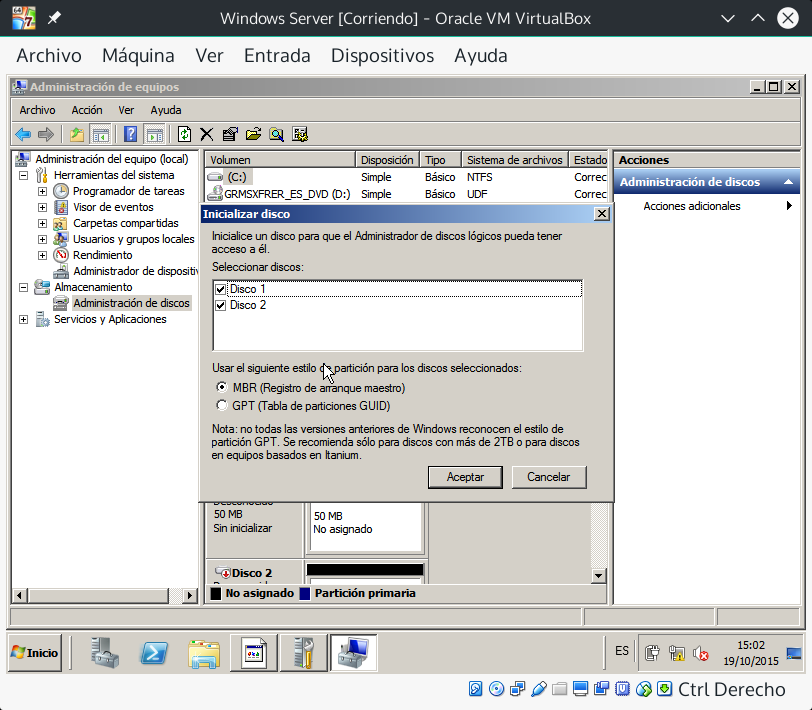
\includegraphics[scale=0.35]{figuras/figura8.png}  %el parámetro scale permite agrandar o achicar la imagen. En el nombre de archivo puede especificar directorios
	\label{figura8}
	
	\caption{Creamos la tabla de particiones} 
\end{figure}
\begin{figure}[H] %con el [H] le obligamos a situar aquí la figura
	\centering
	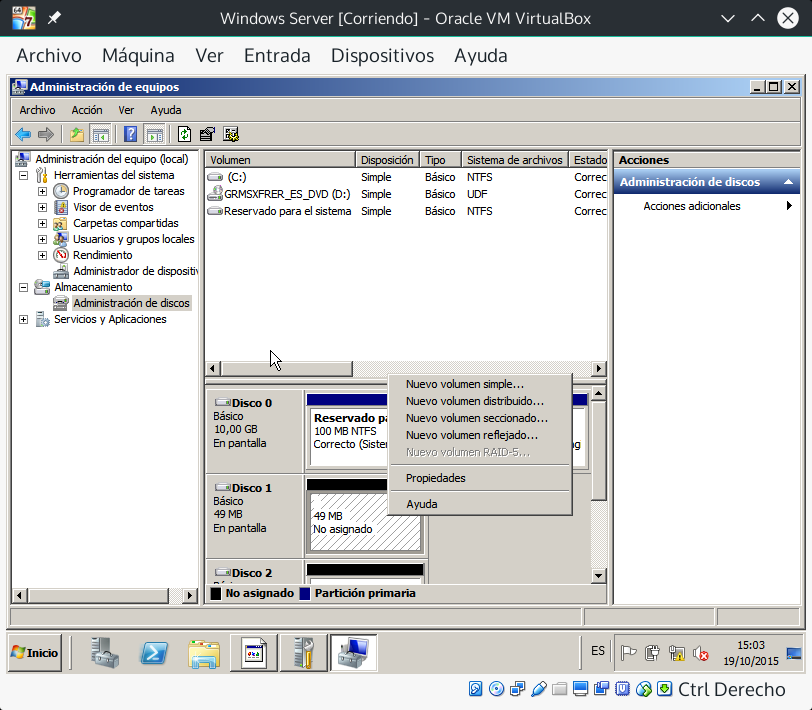
\includegraphics[scale=0.35]{figuras/figura9.png}  %el parámetro scale permite agrandar o achicar la imagen. En el nombre de archivo puede especificar directorios
	\label{figura9}
	
	\caption{Pulsamos con el botón derecho sobre el disco de 50MBi y le damos a Nuevo volúmen reflejado} 
\end{figure}
\begin{figure}[H] %con el [H] le obligamos a situar aquí la figura
	\centering
	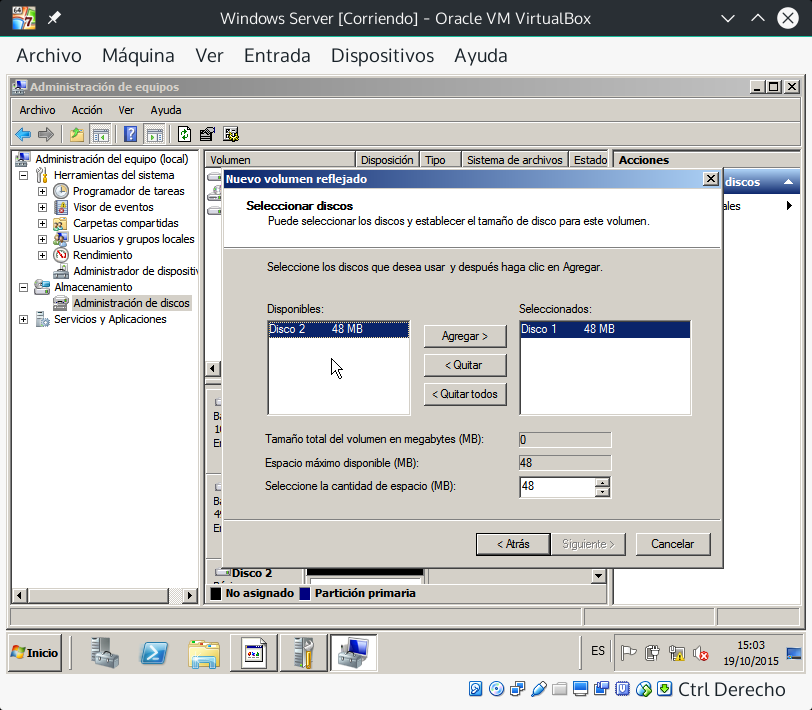
\includegraphics[scale=0.35]{figuras/figura10.png}  %el parámetro scale permite agrandar o achicar la imagen. En el nombre de archivo puede especificar directorios
	\label{figura10}
	
	\caption{Agregamos el Disco 2 también} 
\end{figure}
\begin{figure}[H] %con el [H] le obligamos a situar aquí la figura
	\centering
	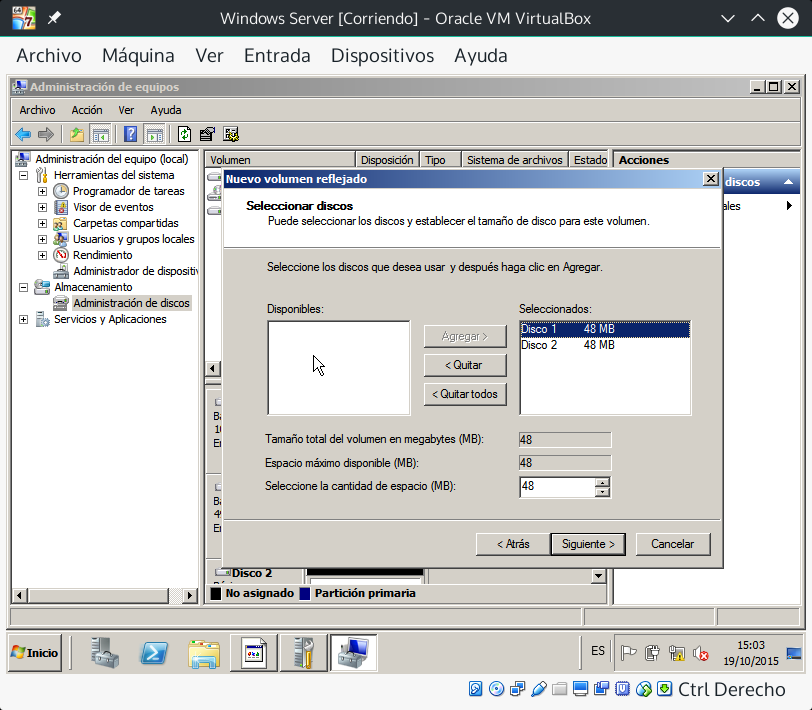
\includegraphics[scale=0.35]{figuras/figura11.png}  %el parámetro scale permite agrandar o achicar la imagen. En el nombre de archivo puede especificar directorios
	\label{figura11}
	
	\caption{Así queda agregado} 
\end{figure}
\begin{figure}[H] %con el [H] le obligamos a situar aquí la figura
	\centering
	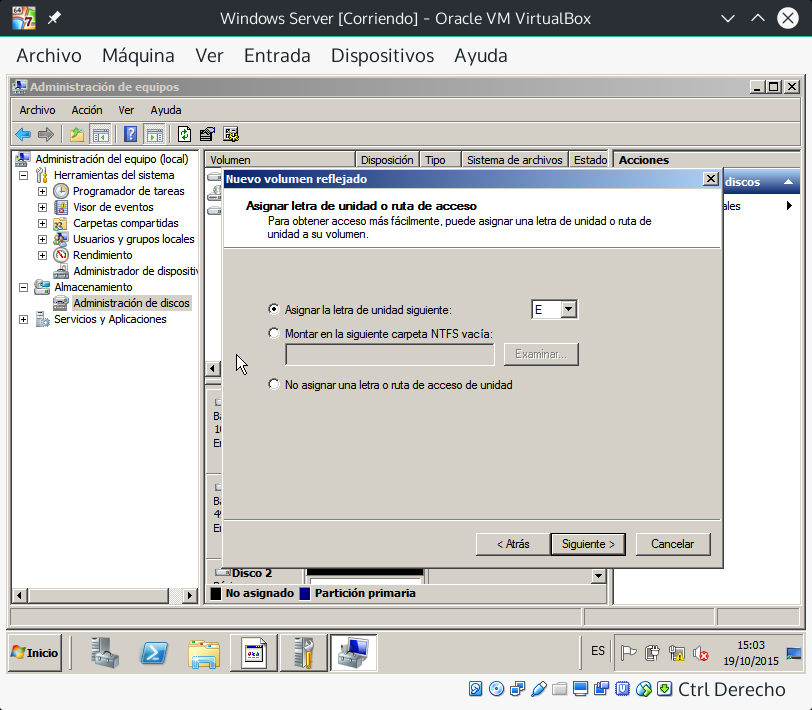
\includegraphics[scale=0.35]{figuras/figura12.png}  %el parámetro scale permite agrandar o achicar la imagen. En el nombre de archivo puede especificar directorios
	\label{figura12}
	
	\caption{Asignamos una letra a la unidad. Yo le he asignado la E} 
\end{figure}
\begin{figure}[H] %con el [H] le obligamos a situar aquí la figura
	\centering
	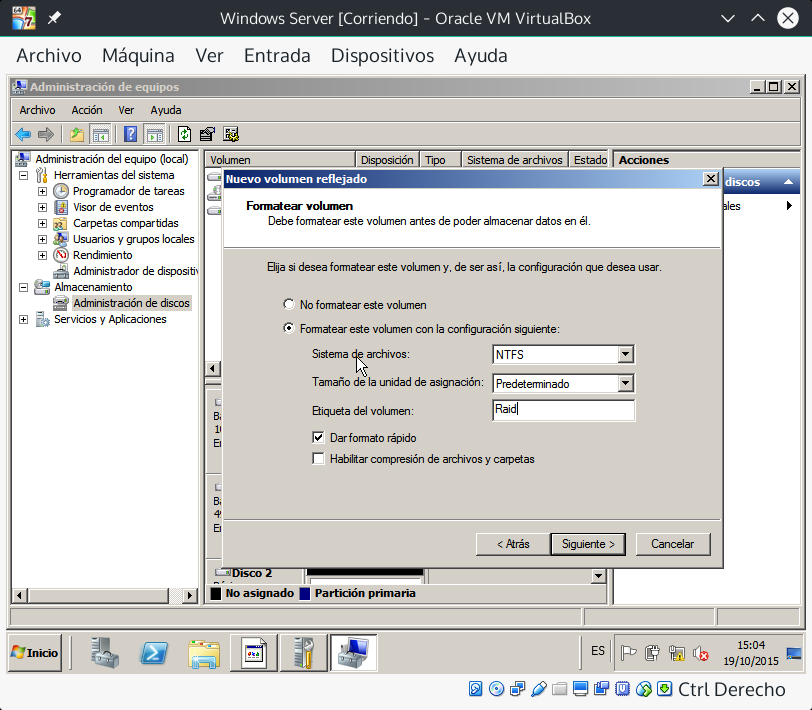
\includegraphics[scale=0.35]{figuras/figura13.png}  %el parámetro scale permite agrandar o achicar la imagen. En el nombre de archivo puede especificar directorios
	\label{figura13}
	
	\caption{Le podemos cambiar la etiqueta al volúmen. Yo la he etiquetado como Raid para que sea más fácil identificarla} 
\end{figure}
\begin{figure}[H] %con el [H] le obligamos a situar aquí la figura
	\centering
	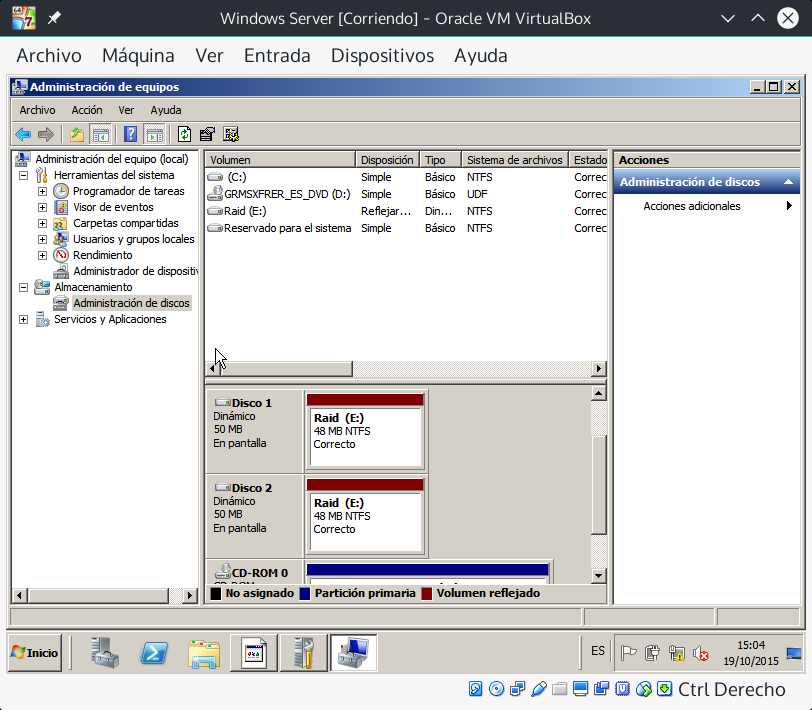
\includegraphics[scale=0.35]{figuras/figura14.png}  %el parámetro scale permite agrandar o achicar la imagen. En el nombre de archivo puede especificar directorios
	\label{figura14}
	
	\caption{Y así quedan configurados los RAID} 
\end{figure}
\section{Cuestión 16: Explique brevemente qué diferencias hay entre los tres tipos de conexión que permite el VMSW para las Mvs: NAT,Host-Only y Bridge}
Según el manual de VirtualBox \cite{natvshstvsbrd} las diferencias serían:
\begin{itemize}
	\item \textbf{NAT: } \textquotedblleft es la forma más sencilla de acceder a una red externa desde una máquina virtual.Normalmente no requiere ninguna configuración en la red del host y el sistema del guest. Por esta razón, es la opción utilizada por defecto en VirtualBox \textquotedblright
	\item \textbf{Host-Only: } \textquotedblleft se puede interpretar como un híbrido los modos de red bridged e interno: como con la red bridged, las máquinas virtuales pueden comunicarse entre ellas y con el host como si estuvieran conectadas por un cable ethernet. Pero como en el modo interno de red, las máquinas virtuales no pueden hablar con el mundo exterior al host ya que no tienen una interfaz de conexión física \textquotedblright
	\begin{figure}[H] %con el [H] le obligamos a situar aquí la figura
		\centering
		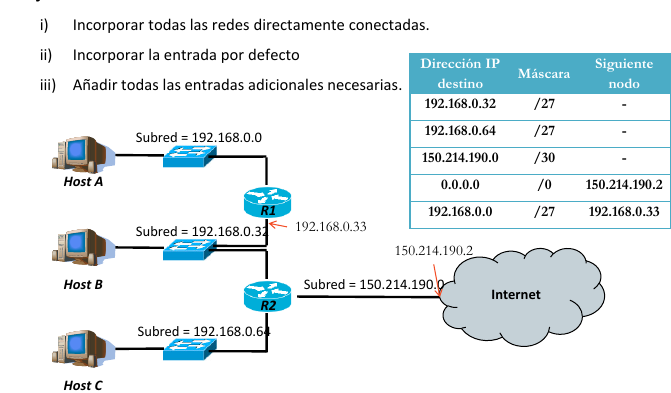
\includegraphics[scale=0.5]{figuras/figura16.png}  %el parámetro scale permite agrandar o achicar la imagen. En el nombre de archivo puede especificar directorios
		\label{figura16}
		
		\caption{Figura de la configuración de Host-Only en la documentación de VMWare \cite{vmwarefigures}} 
	\end{figure}
	\item \textbf{Bridge: } \textquotedblleft usa un dispositivo driver en tu sistema host que filtra los datos de tu adaptador físico de red. Esto permite a VirtualBox interceptar los datos de la red física e inyectarle datos, creando una nueva interfaz de red en el software. \textquotedblright
	\begin{figure}[H] %con el [H] le obligamos a situar aquí la figura
		\centering
		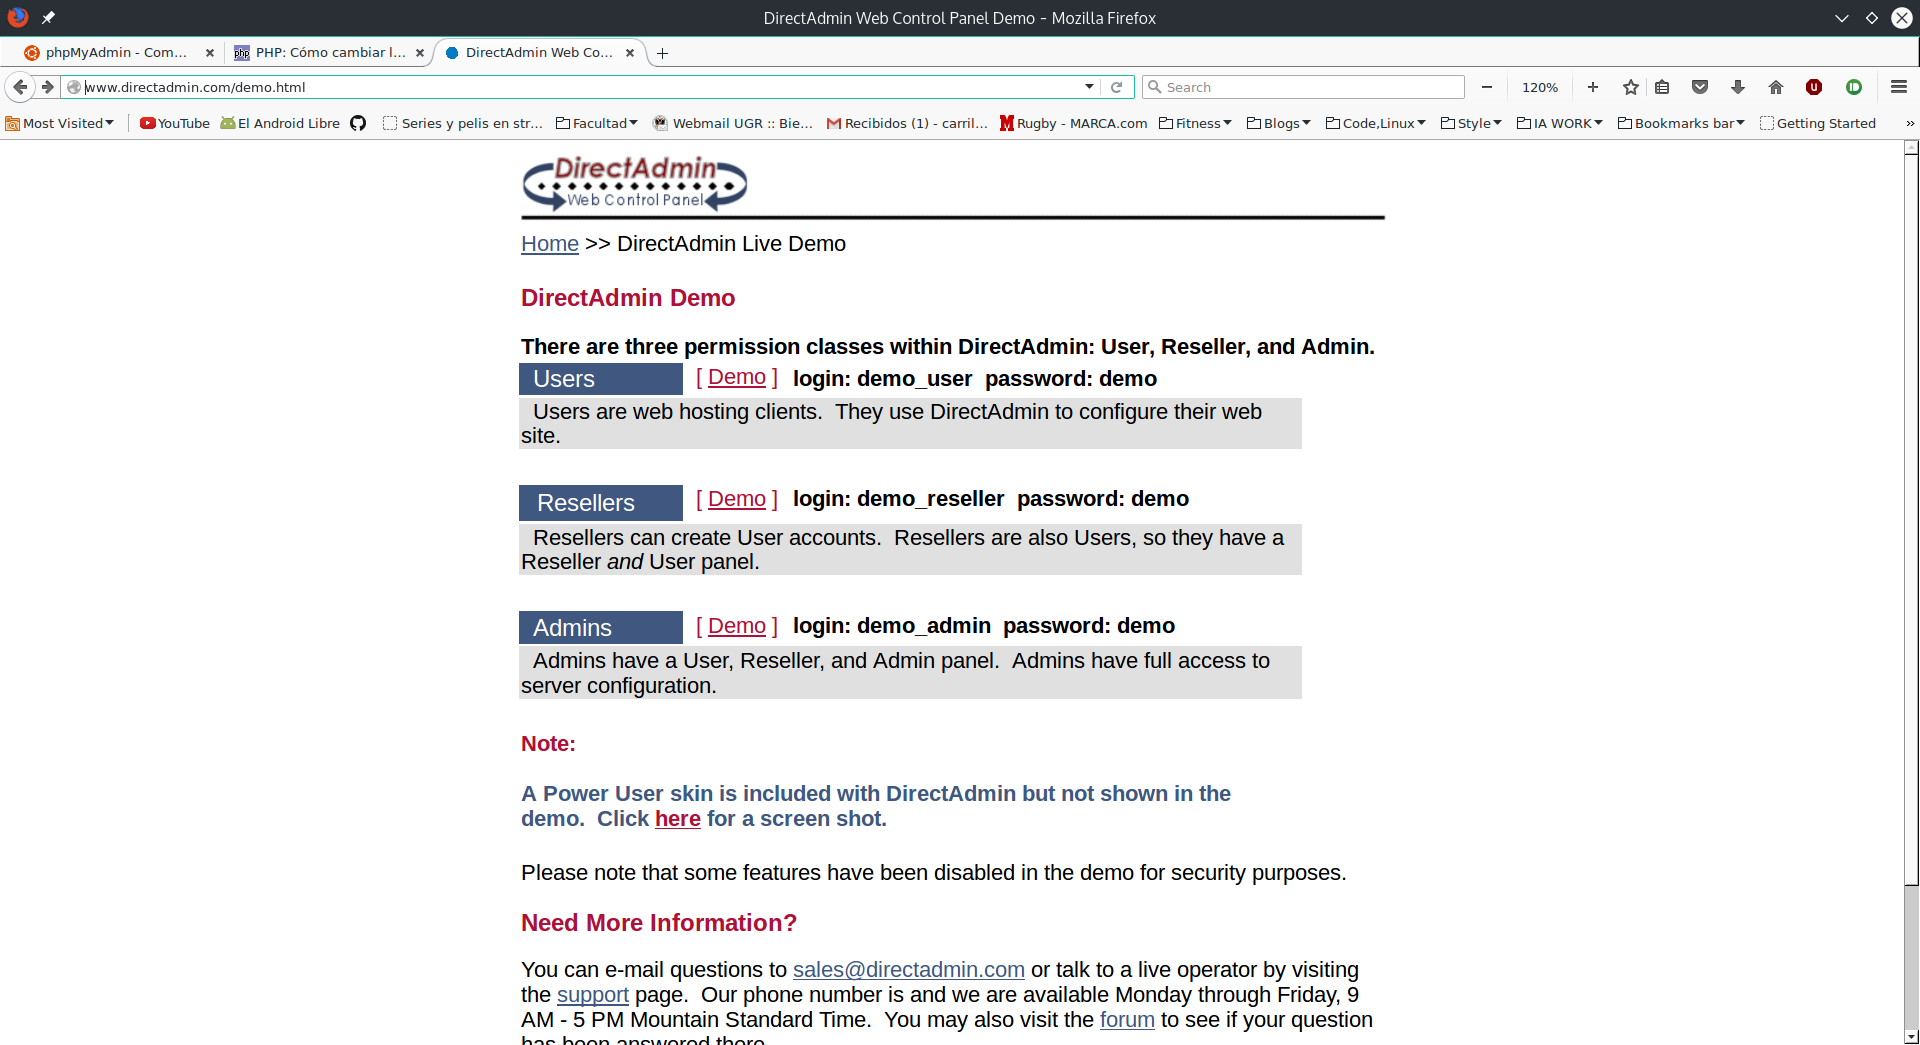
\includegraphics[scale=0.5]{figuras/figura15.png}  %el parámetro scale permite agrandar o achicar la imagen. En el nombre de archivo puede especificar directorios
		\label{figura15}
		
		\caption{Figura de la configuración de Bridged en la documentación de VMWare \cite{vmwarefigures}} 
	\end{figure}
\end{itemize}
\newpage
\bibliography{citas} %archivo citas.bib que contiene las entradas 
\bibliographystyle{ieeetr} % hay varias formas de citar
\end{document}